% !TEX program = pdflatex
\documentclass[11pt,a4paper]{report}

% =====================
%      PREAMBOLO
% =====================
\usepackage[utf8]{inputenc}
\usepackage[T1]{fontenc}
\usepackage{textcomp}
\usepackage{lmodern}
\usepackage[italian]{babel}
\usepackage{geometry}
\geometry{margin=2.5cm}
\usepackage{setspace}
\onehalfspacing
\usepackage{graphicx}
\usepackage{float}
\usepackage{booktabs}
\usepackage{caption}
\usepackage{subcaption}
\usepackage{amsmath, amssymb}
\usepackage{siunitx}
\usepackage{xcolor}
\usepackage{enumitem}
\usepackage{hyperref}
\hypersetup{colorlinks=true,linkcolor=blue,citecolor=blue,urlcolor=blue}
\usepackage{listings}
\usepackage{tcolorbox}
\tcbset{colback=gray!5,colframe=gray!50!black,boxrule=0.5pt,arc=1mm}
\lstset{basicstyle=\ttfamily\small,breaklines=true,frame=tb,numbers=left,numberstyle=\tiny,keywordstyle=\color{blue!70!black},commentstyle=\color{gray!80!black},stringstyle=\color{teal!70!black}}
\graphicspath{{figures/}{selected_figures/}{../immagini/}}


\DeclareUnicodeCharacter{2212}{-} % sostituisce il "meno" Unicode con un normale trattino
\DeclareUnicodeCharacter{00A0}{ } % sostituisce lo spazio non separabile
\DeclareUnicodeCharacter{2013}{--} % trattino medio
\DeclareUnicodeCharacter{2014}{---} % trattino lungo




% Comandi utili
\newcommand{\dataset}{\texttt{Flickr8k}}
\newcommand{\bos}{\texttt{<bos>}}
\newcommand{\eos}{\texttt{<eos>}}
\newcommand{\pad}{\texttt{<pad>}}
\newcommand{\unk}{\texttt{<unk>}}

\begin{document}

% =====================
%     FRONT MATTER
% =====================
\begin{titlepage}
  \centering

  % Logo Università di Parma
  \IfFileExists{../immagini/logo_unipr.png}{\includegraphics[width=0.50\textwidth]{../immagini/logo_unipr.png}\\[1.2 em]}{}  
  
  {\Large \textbf{Università degli Studi di Parma} \\[0.3em]
  \textbf{Corso di Laurea Magistrale in Ingegneria Informatica} \\[0.3em]
  Curriculum: \textbf{Intelligenza Artificiale} \\[2em]}
  
  {\Huge \textbf{Image Captioning con CNN--LSTM su Flickr8k}}\\[0.8em]
  
  \rule{\linewidth}{0.4pt}\\[0.8em]
  \textbf{Obiettivo:} 
  Il presente elaborato analizza e spiega in modo approfondito l’assegnamento n.\,27 del corso di \emph{Deep Learning e Modelli Generativi}, che richiede lo sviluppo di un sistema di \emph{image captioning} capace di generare automaticamente descrizioni testuali a partire da immagini di input.  
  Il modello proposto si basa su un’architettura ibrida \textbf{CNN--LSTM}, in cui la rete convoluzionale estrae le caratteristiche visive e la rete LSTM produce la sequenza linguistica corrispondente.  
  L’intero progetto è stato realizzato in \textbf{PyTorch}, con l’obiettivo di costruire un sistema completo, chiaro e replicabile per lo studio e la comprensione del processo di generazione automatica di didascalie.\\[0.8em]
  \rule{\linewidth}{0.4pt}\\[4em]
  
  \begin{tabular}{ll}
  Studente: & Giuseppe Dimonte \\
  Docente: & Prof. Andrea Prati \\
  Corso: & Deep Learning e Modelli Generativi \\
  \end{tabular}
\end{titlepage}

% =====================
%       ABSTRACT (IT)
% =====================
\begin{abstract}
Il presente elaborato descrive lo sviluppo di un sistema di \emph{image captioning}, il cui obiettivo è generare automaticamente una descrizione testuale coerente e significativa a partire da un’immagine di input.  
Il lavoro si basa sull’assegnamento n.\,27 del corso di \emph{Deep Learning e Modelli Generativi} e utilizza il dataset pubblico \dataset{}, costituito da 8.000 immagini, ognuna associata a cinque didascalie scritte da persone diverse.

L’architettura implementata combina una rete neurale convoluzionale (CNN) per l’estrazione delle caratteristiche visive con una rete LSTM (\emph{Long Short-Term Memory}) per la generazione sequenziale delle parole, secondo il paradigma \emph{image-to-sequence}.  
Durante l’addestramento sono state adottate tecniche di ottimizzazione avanzate, come \emph{teacher forcing}, \emph{scheduled sampling}, \emph{label smoothing} e \emph{gradient clipping}, al fine di migliorare la stabilità e la qualità delle didascalie generate.

Il documento illustra in modo dettagliato tutte le fasi del progetto — dalla pulizia e codifica dei dati, alla costruzione del modello e alla valutazione tramite la metrica BLEU — con l’obiettivo di fornire una visione completa, didattica e replicabile del processo di generazione automatica di descrizioni visive.
\end{abstract}


\chapter{Introduzione}

\section{Perché l'image captioning?}

Immaginate di mostrare una fotografia a un assistente digitale e ricevere immediatamente una descrizione testuale chiara, corretta e coerente: questo è l’obiettivo dell’\emph{image captioning}.  
Si tratta di una delle applicazioni più rappresentative dell’intelligenza artificiale moderna, poiché unisce la \textbf{comprensione visiva} (tipica delle reti convoluzionali) alla \textbf{generazione linguistica} (tipica dei modelli sequenziali o di linguaggio).

L’importanza di questa disciplina è molteplice:
\begin{itemize}
  \item \textbf{Accessibilità}: un sistema in grado di descrivere automaticamente immagini può aiutare persone ipovedenti a comprendere il contenuto visivo di fotografie, video o pagine web.
  \item \textbf{Organizzazione dei contenuti}: nelle grandi piattaforme di immagini (come Flickr, Google Photos o Instagram), generare descrizioni automatiche aiuta a migliorare la ricerca e l’indicizzazione.
  \item \textbf{Sistemi multimodali}: l’image captioning è una componente essenziale in sistemi che combinano visione e linguaggio, come i modelli \emph{Vision-Language}, i chatbot visivi o i generatori di testo condizionati da immagini.
\end{itemize}

Inoltre, l’image captioning rappresenta un eccellente banco di prova per il \textbf{deep learning multimodale}, perché obbliga il modello a combinare due forme di informazione profondamente diverse: i pixel e le parole.  
Questo comporta non solo un problema di apprendimento supervisionato, ma anche una sfida cognitiva: tradurre il linguaggio visivo in linguaggio naturale.

\begin{tcolorbox}[title=Messaggio chiave]
L'image captioning è il punto d'incontro tra la visione artificiale e l'elaborazione del linguaggio naturale: un modello che “vede” come un umano e “parla” come un umano.
\end{tcolorbox}


\section{Contesto del progetto}

Il lavoro qui presentato si inserisce nell’ambito del corso di \emph{Deep Learning e Modelli Generativi}, ed è relativo all’assegnamento n.\,27.  
L’obiettivo dell’assegnamento è lo sviluppo, in \textbf{PyTorch}, di un sistema completo di image captioning capace di:
\begin{enumerate}
  \item estrarre le caratteristiche visive salienti da un’immagine tramite una rete neurale convoluzionale (CNN);
  \item utilizzare tali informazioni come contesto per una rete LSTM (Long Short-Term Memory), che genera una frase parola per parola;
  \item decodificare la sequenza di parole in linguaggio naturale grazie a un classificatore finale (MLP).
\end{enumerate}

Il dataset utilizzato è \dataset{}, una raccolta di 8.000 immagini annotate con cinque descrizioni testuali ciascuna.  
Tale dataset è spesso impiegato come benchmark per modelli di captioning di piccola scala, poiché consente di sperimentare con architetture relativamente leggere ma efficaci.

Il progetto richiede non solo di implementare la pipeline di addestramento e valutazione, ma anche di comprendere a fondo le scelte architetturali, la gestione dei dati, le metriche di qualità e le strategie di ottimizzazione.

\section{Idea di base}

La pipeline alla base del sistema può essere riassunta in tre passaggi fondamentali:

\begin{enumerate}
  \item \textbf{Feature extraction:} una \textbf{CNN}, pre-addestrata su un grande dataset come ImageNet, trasforma l’immagine in un vettore di caratteristiche numeriche (\emph{feature vector}) che rappresentano il contenuto visivo in forma compatta.
  \item \textbf{Sequenza linguistica:} una \textbf{LSTM} riceve questo vettore come stato iniziale e genera la didascalia parola per parola, apprendendo la correlazione tra caratteristiche visive e parole del linguaggio naturale.
  \item \textbf{Decodifica finale:} un piccolo \textbf{MLP} (Multi-Layer Perceptron) trasforma lo stato nascosto della LSTM in una distribuzione di probabilità sulle parole del vocabolario, scegliendo quella più probabile a ogni passo.
\end{enumerate}

\begin{tcolorbox}[title=Messaggio chiave]
Le CNN “vedono”, le LSTM “parlano”.  
La CNN comprime il contenuto visivo in un vettore, la LSTM lo utilizza per costruire una frase coerente e plausibile che descriva ciò che l’immagine rappresenta.
\end{tcolorbox}


\section{Obiettivi didattici}

Oltre all’aspetto implementativo, questo progetto ha anche una forte valenza formativa:
\begin{itemize}
  \item comprendere come modelli differenti (CNN e LSTM) possano essere integrati in un’unica pipeline;
  \item imparare a gestire dataset multimodali (immagini + testo);
  \item applicare tecniche di pre-processing e tokenizzazione del linguaggio;
  \item sperimentare metodi di ottimizzazione e regolarizzazione tipici del deep learning moderno;
  \item interpretare le metriche di valutazione come BLEU e analizzare qualitativamente le caption generate.
\end{itemize}

Questo elaborato, pertanto, non si limita a presentare un modello funzionante, ma mira a fornire una spiegazione esaustiva, passo per passo, dell’intero processo di costruzione di un sistema di image captioning moderno e riproducibile.


\chapter{Il Dataset Flickr8k}

\section{Introduzione al dataset}

Per addestrare un modello di \emph{image captioning} è necessario disporre di un dataset che colleghi il dominio visivo (le immagini) a quello linguistico (le descrizioni testuali).  
Il dataset scelto per questo progetto è \textbf{Flickr8k}, una raccolta pubblica ampiamente utilizzata nella ricerca accademica per modelli di generazione automatica di didascalie.

Il dataset, originariamente sviluppato presso la University of Illinois, contiene:
\begin{itemize}
  \item \textbf{8.000 immagini} di scene naturali (persone, animali, oggetti, attività);
  \item \textbf{5 descrizioni testuali per ciascuna immagine}, scritte manualmente da annotatori umani;
  \item una suddivisione ufficiale in \emph{training set}, \emph{validation set} e \emph{test set}.
\end{itemize}

Le immagini provengono dal sito web \emph{Flickr.com} e rappresentano situazioni della vita quotidiana: bambini che giocano, animali in movimento, persone impegnate in attività sportive o ricreative.  
Le descrizioni testuali, o \emph{caption}, offrono un breve riassunto del contenuto visivo espresso in linguaggio naturale. Ad esempio:

\begin{tcolorbox}[title=Esempio di didascalia]
\textbf{Immagine:} un cane che corre su un prato.\\[0.3em]
\textbf{Didascalie associate:}
\begin{itemize}
  \item A brown dog is running through the grass.
  \item The dog runs across a grassy field.
  \item A dog is playing outside on the grass.
  \item The brown dog is in motion.
  \item A dog runs through a green field.
\end{itemize}
\end{tcolorbox}

Come si può osservare, le descrizioni non sono identiche ma esprimono lo stesso concetto con parole diverse.  
Questo aspetto è cruciale, poiché durante l’addestramento il modello apprende non solo la relazione tra immagine e testo, ma anche la varietà linguistica con cui è possibile descrivere la stessa scena.

\section{Struttura dei file}

Dopo aver scaricato il dataset (ad esempio dal repository GitHub \href{https://github.com/goodwillyoga/Flickr8k_dataset}{goodwillyoga/Flickr8k\_dataset}), la struttura delle cartelle appare come segue:

\begin{verbatim}
Flickr8k_Dataset/
|-- Flickr8k_Dataset/         # Contiene tutte le immagini (.jpg)
|-- Flickr8k_text/
|   |-- Flickr8k.token.txt    # Tutte le descrizioni
|   |-- Flickr_8k.trainImages.txt
|   |-- Flickr_8k.testImages.txt
|   \-- Flickr_8k.devImages.txt
\end{verbatim}

Il file \texttt{Flickr8k.token.txt} contiene tutte le associazioni tra immagini e descrizioni.  
Ogni riga segue il formato:

\begin{verbatim}
1000268201_693b08cb0e.jpg#0  A child in a pink dress is climbing up a set of stairs.
1000268201_693b08cb0e.jpg#1  A girl going into a wooden building.
\end{verbatim}

Dove:
\begin{itemize}
  \item la parte prima del simbolo “\#” indica il nome dell’immagine;
  \item il numero dopo “\#” rappresenta l’indice progressivo della descrizione (da 0 a 4);
  \item dopo uno spazio segue la didascalia vera e propria.
\end{itemize}

\section{Pulizia del testo e pre-processing}

Prima di poter addestrare una rete neurale, le frasi devono essere trasformate in una rappresentazione numerica.  
Il primo passo consiste nella \textbf{pulizia del testo}, che serve a uniformare le descrizioni e ridurre la variabilità inutile.

Le principali operazioni di pulizia sono:
\begin{itemize}
  \item conversione di tutte le parole in minuscolo;
  \item rimozione di numeri e punteggiatura;
  \item eliminazione di parole composte da un solo carattere (es. “a”, “s”);
  \item rimozione di spazi multipli o finali.
\end{itemize}

\begin{lstlisting}[language=Python, caption={Funzione di pulizia del testo delle caption.}]
import re

def clean_caption(text):
    """
    Pulisce una didascalia secondo le regole del progetto.
    """
    text = text.lower()                       # converte tutto in minuscolo
    text = re.sub(r"[^a-z\\s]", "", text)     # rimuove numeri e punteggiatura
    words = [w for w in text.split() if len(w) > 1]  # elimina parole di 1 carattere
    return " ".join(words)
\end{lstlisting}

\begin{tcolorbox}[title=Spiegazione ]
\begin{itemize}
  \item \texttt{lower()} converte l’intera frase in minuscolo per evitare duplicazioni come “Dog” e “dog”.
  \item \texttt{re.sub(...)} rimuove simboli, cifre e punteggiatura.
  \item La list comprehension elimina parole corte e non significative.
  \item Infine, si ricostruisce la frase pulita.
\end{itemize}
\end{tcolorbox}

Dopo la pulizia, si crea un dizionario Python che associa a ogni immagine le sue cinque descrizioni pulite:

\begin{lstlisting}[language=Python, caption={Creazione del dizionario delle caption.}]
captions_dict = {}

for line in open("Flickr8k_text/Flickr8k.token.txt"):
    image_id, caption = line.split("\t")
    image_id = image_id.split("#")[0]
    caption = clean_caption(caption)
    captions_dict.setdefault(image_id, []).append(caption)
\end{lstlisting}

\begin{tcolorbox}[title=Struttura del dizionario]
Ogni chiave del dizionario (\texttt{image\_id}) corrisponde al nome di un file immagine, e il valore associato è una lista di cinque frasi pulite.  
Questo formato verrà utilizzato successivamente per creare il dataset PyTorch personalizzato.
\end{tcolorbox}

\section{Costruzione del vocabolario}

Dopo la pulizia, le parole devono essere convertite in numeri.  
Ogni parola del dataset viene quindi mappata a un indice intero all’interno di un \textbf{vocabolario}.  
Il vocabolario è costruito includendo solo le parole che compaiono almeno un certo numero di volte (ad esempio 5), per ridurre la dimensione del dizionario e migliorare la generalizzazione.

Vengono aggiunti inoltre quattro token speciali:
\begin{itemize}
  \item \bos{} — inizio della frase;
  \item \eos{} — fine della frase;
  \item \pad{} — padding per uniformare la lunghezza delle sequenze;
  \item \unk{} — parole non presenti nel vocabolario.
\end{itemize}

\begin{lstlisting}[language=Python, caption={Costruzione del vocabolario.}]
from collections import Counter

counter = Counter()
for caps in captions_dict.values():
    for c in caps:
        counter.update(c.split())

vocab = [word for word, count in counter.items() if count >= 5]
vocab = ["<pad>", "<bos>", "<eos>", "<unk>"] + sorted(vocab)
word2idx = {w: i for i, w in enumerate(vocab)}
idx2word = {i: w for w, i in word2idx.items()}
\end{lstlisting}

\begin{tcolorbox}[title=Nota]
Il dizionario \texttt{word2idx} verrà salvato in un file (ad esempio \texttt{vocab.json}) per essere caricato durante l’addestramento.  
Impostare una soglia minima di frequenza (come 5 occorrenze) aiuta a ridurre la complessità del modello e a limitare l’overfitting su parole rare.
\end{tcolorbox}

\section{Riepilogo}

In questo capitolo abbiamo:
\begin{itemize}
  \item esplorato la struttura del dataset \dataset{};
  \item compreso il formato dei file e delle descrizioni;
  \item pulito e normalizzato il testo delle caption;
  \item costruito un dizionario e un vocabolario numerico.
\end{itemize}

Questi passaggi costituiscono la base per la fase successiva: la creazione del \textbf{dataset personalizzato PyTorch}, che collegherà in modo efficiente le immagini preprocessate e le didascalie tokenizzate.

\begin{tcolorbox}[title=Riferimento al codice]
Nel repository finale, la preparazione dei dati è stata consolidata negli script \texttt{src/vocab\_builder.py} e \texttt{src/prepare\_data.py}, utilizzati per generare il vocabolario e gli split effettivamente impiegati negli esperimenti.
\end{tcolorbox}


\chapter{Fondamenti di Deep Learning}

\section{Dai neuroni artificiali alle reti profonde}

Il \emph{deep learning} è un ramo dell’apprendimento automatico che utilizza reti neurali multistrato per apprendere relazioni complesse a partire dai dati.  
Il blocco fondamentale di una rete neurale è il \textbf{neurone artificiale}, che rappresenta una versione semplificata del neurone biologico.

Ogni neurone riceve uno o più input numerici, li moltiplica per pesi associati, aggiunge un termine di bias e applica una funzione di attivazione non lineare:

\begin{equation}
y = f(\mathbf{w}^\top \mathbf{x} + b)
\end{equation}

dove:
\begin{itemize}
  \item $\mathbf{x}$ è il vettore degli input;
  \item $\mathbf{w}$ rappresenta i pesi appresi durante l’addestramento;
  \item $b$ è il bias, un termine aggiuntivo per spostare la funzione di attivazione;
  \item $f(\cdot)$ è la funzione di attivazione (ad esempio ReLU o sigmoid).
\end{itemize}

La funzione di attivazione introduce una componente non lineare nel modello, permettendo alla rete di rappresentare relazioni complesse che non possono essere catturate da modelli puramente lineari.

\begin{tcolorbox}[title=Idea chiave]
Senza funzioni di attivazione non lineari, anche più strati di neuroni si ridurrebbero a un’unica trasformazione lineare: la rete non sarebbe in grado di apprendere relazioni complesse tra i dati.
\end{tcolorbox}

\section{Architettura di una rete neurale}

Una rete neurale profonda (DNN, \emph{Deep Neural Network}) è costruita impilando più strati di neuroni, in modo che ciascun livello apprenda una rappresentazione progressivamente più astratta dei dati.

\begin{itemize}
  \item \textbf{Strato di input:} riceve i dati grezzi (ad esempio i pixel di un’immagine o le parole codificate come numeri).
  \item \textbf{Strati nascosti:} elaborano rappresentazioni intermedie tramite moltiplicazioni di matrici e funzioni di attivazione.
  \item \textbf{Strato di output:} produce il risultato finale, come una classe o una sequenza di parole.
\end{itemize}

Un esempio minimale di rete neurale in PyTorch può essere scritto così:

\begin{lstlisting}[language=Python, caption={Esempio di rete neurale feed-forward in PyTorch.}]
import torch
import torch.nn as nn

class SimpleNet(nn.Module):
    def __init__(self, input_dim, hidden_dim, output_dim):
        super(SimpleNet, self).__init__()
        self.fc1 = nn.Linear(input_dim, hidden_dim)
        self.relu = nn.ReLU()
        self.fc2 = nn.Linear(hidden_dim, output_dim)

    def forward(self, x):
        x = self.relu(self.fc1(x))
        return self.fc2(x)
\end{lstlisting}

\begin{tcolorbox}[title=Spiegazione]
Questa piccola rete è composta da due strati lineari separati da una funzione di attivazione ReLU.  
Durante l’addestramento, la rete apprende i valori dei pesi all’interno di \texttt{fc1} e \texttt{fc2} per minimizzare l’errore di predizione.
\end{tcolorbox}

\section{Il processo di addestramento}

L’obiettivo dell’addestramento di una rete neurale è trovare l’insieme di pesi che minimizza una data \textbf{funzione di perdita} (\emph{loss function}) — cioè una misura dell’errore tra le predizioni del modello e i valori corretti.

Il processo tipico di addestramento segue questi passaggi:
\begin{enumerate}
  \item Eseguire una \textbf{forward pass} per calcolare le predizioni.
  \item Calcolare la \textbf{funzione di perdita} (es. entropia incrociata o errore quadratico medio).
  \item Calcolare il gradiente della perdita rispetto ai pesi tramite la \textbf{backpropagation}.
  \item Aggiornare i pesi usando un algoritmo di ottimizzazione come \textbf{Stochastic Gradient Descent (SGD)} o \textbf{Adam}.
\end{enumerate}

In PyTorch, un singolo passo di ottimizzazione può essere riassunto così:

\begin{lstlisting}[language=Python, caption={Esempio di passo di ottimizzazione in PyTorch.}]
optimizer.zero_grad()       # azzera i gradienti accumulati
outputs = model(inputs)     # forward pass
loss = criterion(outputs, targets)  # calcola la loss
loss.backward()             # backpropagation
optimizer.step()            # aggiorna i pesi
\end{lstlisting}

\begin{tcolorbox}[title=Concetto: discesa del gradiente]
La discesa del gradiente aggiorna ciascun peso nella direzione che riduce la perdita:
\[
w := w - \eta \frac{\partial L}{\partial w}
\]
dove $\eta$ è il tasso di apprendimento (\emph{learning rate}), un iperparametro che controlla l’ampiezza del passo di aggiornamento.
\end{tcolorbox}

\section{Epoche, batch e iterazioni}

L’addestramento delle reti neurali avviene tipicamente in più cicli chiamati \textbf{epoche}.  
Un’epoca corrisponde al momento in cui il modello ha visto l’intero dataset una volta.  
Poiché elaborare tutto il dataset in un unico blocco sarebbe inefficiente, si divide il set di dati in sottoinsiemi più piccoli chiamati \textbf{batch}.

\begin{itemize}
  \item Ogni \textbf{batch} contiene un piccolo gruppo di esempi (ad esempio 32 o 64).
  \item Una \textbf{iterazione} corrisponde a un aggiornamento dei pesi basato su un singolo batch.
  \item Dopo aver elaborato tutti i batch, si completa un’epoca.
\end{itemize}

\begin{tcolorbox}[title=Esempio]
Se il dataset contiene 8.000 campioni e la dimensione del batch è 64, allora ogni epoca è composta da $\frac{8000}{64} \approx 125$ iterazioni.
\end{tcolorbox}

Capire la relazione tra epoche, batch e iterazioni è fondamentale per regolare l’addestramento e prevenire problemi come \emph{overfitting} o \emph{underfitting}.

\section{Overfitting e regolarizzazione}

Un problema comune nel deep learning è l’\textbf{overfitting}, che si verifica quando il modello impara troppo bene i dati di addestramento ma fallisce nel generalizzare su dati nuovi.  
In pratica, il modello “memorizza” anziché “apprendere”.

Per contrastarlo, si utilizzano varie tecniche di \textbf{regolarizzazione}:
\begin{itemize}
  \item \textbf{Dropout:} disattiva casualmente alcuni neuroni durante l’addestramento per evitare co-adattamenti.
  \item \textbf{Weight decay:} penalizza pesi troppo grandi mediante una regolarizzazione $L_2$.
  \item \textbf{Early stopping:} interrompe l’addestramento quando la perdita di validazione smette di migliorare.
  \item \textbf{Data augmentation:} aumenta la varietà dei dati applicando trasformazioni alle immagini (rotazioni, tagli, flip, ecc.).
\end{itemize}

\begin{tcolorbox}[title=Nota pratica]
Nel progetto Flickr8k, tecniche come \emph{dropout} ed \emph{early stopping} vengono applicate per migliorare la capacità di generalizzazione del modello CNN–LSTM.
\end{tcolorbox}

\section{Funzioni di perdita e algoritmi di ottimizzazione}

La scelta della funzione di perdita dipende dal tipo di problema:
\begin{itemize}
  \item \textbf{Cross-Entropy Loss:} usata per classificazione o generazione di sequenze (come la caption di un’immagine).
  \item \textbf{Mean Squared Error (MSE):} usata per problemi di regressione.
\end{itemize}

Gli algoritmi di ottimizzazione più diffusi includono:
\begin{itemize}
  \item \textbf{SGD (Stochastic Gradient Descent):} semplice ed efficace, aggiorna i pesi a piccoli passi.
  \item \textbf{Adam:} versione adattiva dell’SGD, adatta dinamicamente il learning rate per ogni parametro.
  \item \textbf{RMSProp:} simile ad Adam, particolarmente efficace per reti ricorrenti.
\end{itemize}

\begin{lstlisting}[language=Python, caption={Definizione della funzione di perdita e dell’ottimizzatore in PyTorch.}]
criterion = nn.CrossEntropyLoss()
optimizer = torch.optim.Adam(model.parameters(), lr=1e-3)
\end{lstlisting}

\section{Riepilogo}

In questo capitolo sono stati introdotti i concetti fondamentali del deep learning che costituiscono la base teorica del modello CNN–LSTM sviluppato nei capitoli successivi:
\begin{itemize}
  \item la struttura delle reti neurali e il ruolo delle funzioni di attivazione;
  \item il ciclo di addestramento, la backpropagation e l’ottimizzazione;
  \item il significato di epoca, batch e iterazione;
  \item le principali tecniche di regolarizzazione per migliorare la generalizzazione.
\end{itemize}

Queste basi teoriche sono indispensabili per comprendere come nei prossimi capitoli — dedicati a CNN e LSTM — i due mondi della visione artificiale e del linguaggio naturale vengano integrati in un unico modello coerente.

\begin{tcolorbox}[title=Riferimento al codice]
I frammenti di codice di esempio di questo capitolo hanno valore illustrativo; nel repository finale, i file realmente coinvolti nella pipeline sono \texttt{src/dataset.py}, \texttt{src/model.py}, \texttt{src/train.py}, \texttt{src/eval.py} e \texttt{src/visualize.py}.
\end{tcolorbox}


\chapter{Reti Neurali Convoluzionali (CNN)}

\section{Introduzione alle CNN}

Le \textbf{reti neurali convoluzionali} (\emph{Convolutional Neural Networks}, CNN) rappresentano il cuore della moderna visione artificiale.  
Sono progettate per estrarre automaticamente caratteristiche visive (\emph{features}) da immagini, riconoscendo pattern spaziali come bordi, forme, colori e oggetti.

A differenza delle reti completamente connesse, dove ogni neurone è collegato a tutti gli input, una CNN sfrutta la struttura locale dei dati visivi: un pixel è influenzato principalmente dai pixel vicini.  
Questo principio riduce il numero di parametri e migliora l’efficienza.

\begin{tcolorbox}[title=Idea chiave]
Le CNN imparano a “vedere” come l’occhio umano: nei primi strati riconoscono bordi e texture, negli strati più profondi identificano oggetti complessi e concetti semantici.
\end{tcolorbox}

\section{Operazione di convoluzione}

L’operazione fondamentale di una CNN è la \textbf{convoluzione}, che consiste nel far scorrere un piccolo filtro (detto anche \emph{kernel}) su tutta l’immagine per estrarne caratteristiche locali.

Matematicamente, per un’immagine $I$ e un filtro $K$ di dimensione $m \times n$, la convoluzione è definita come:

\[
S(i, j) = (I * K)(i, j) = \sum_m \sum_n I(i+m, j+n) \cdot K(m, n)
\]

Il risultato, chiamato \textbf{feature map}, indica quanto un certo pattern (il filtro) è presente in ogni regione dell’immagine.

In PyTorch, un livello convoluzionale può essere definito in modo molto semplice:

\begin{lstlisting}[language=Python, caption={Esempio di layer convoluzionale in PyTorch.}]
import torch
import torch.nn as nn

conv = nn.Conv2d(in_channels=3, out_channels=16, kernel_size=3, stride=1, padding=1)
x = torch.randn(1, 3, 224, 224)  # batch=1, canali=3, immagine 224x224
y = conv(x)
print(y.shape)  # -> torch.Size([1, 16, 224, 224])
\end{lstlisting}

\begin{tcolorbox}[title=Spiegazione]
Il layer convoluzionale riceve un’immagine RGB (3 canali) e applica 16 filtri $3\times3$.  
Il risultato è una rappresentazione dell’immagine con 16 canali, ognuno dei quali evidenzia una diversa caratteristica visiva appresa.
\end{tcolorbox}

\section{Pooling e riduzione dimensionale}

Dopo la convoluzione, è comune applicare un’operazione di \textbf{pooling}, che riduce la dimensione spaziale delle feature map mantenendo le informazioni più rilevanti.  
Il tipo più usato è il \textbf{max pooling}, che conserva solo il valore massimo all’interno di una finestra locale.

\begin{lstlisting}[language=Python, caption={Esempio di operazione di max pooling.}]
pool = nn.MaxPool2d(kernel_size=2, stride=2)
out = pool(y)
print(out.shape)  # -> torch.Size([1, 16, 112, 112])
\end{lstlisting}

\begin{tcolorbox}[title=Effetto del pooling]
La risoluzione spaziale è dimezzata (da 224x224 a 112x112), ma la rete conserva le caratteristiche più significative.  
Questo migliora la robustezza e riduce il numero di parametri.
\end{tcolorbox}

\section{Funzioni di attivazione nelle CNN}

Ogni strato convoluzionale è seguito da una funzione di attivazione non lineare, solitamente la \textbf{ReLU (Rectified Linear Unit)}:

\[
f(x) = \max(0, x)
\]

La ReLU accelera l’addestramento e riduce il problema del gradiente che svanisce.  
In PyTorch, viene integrata direttamente nel flusso della rete:

\begin{lstlisting}[language=Python, caption={Uso della funzione ReLU in una CNN.}]
model = nn.Sequential(
    nn.Conv2d(3, 16, 3, 1, 1),
    nn.ReLU(),
    nn.MaxPool2d(2, 2)
)
\end{lstlisting}

\section{Struttura generale di una CNN}

Una CNN completa combina più livelli convoluzionali, di pooling e non linearità.  
Negli ultimi strati, le feature vengono “appiattite” in un vettore e passate a uno o più strati lineari (\emph{fully connected}) per la classificazione o altre predizioni.

\begin{lstlisting}[language=Python, caption={Esempio di CNN semplificata.}]
class SimpleCNN(nn.Module):
    def __init__(self):
        super(SimpleCNN, self).__init__()
        self.features = nn.Sequential(
            nn.Conv2d(3, 32, 3, 1, 1),
            nn.ReLU(),
            nn.MaxPool2d(2),
            nn.Conv2d(32, 64, 3, 1, 1),
            nn.ReLU(),
            nn.MaxPool2d(2)
        )
        self.classifier = nn.Sequential(
            nn.Linear(64 * 56 * 56, 256),
            nn.ReLU(),
            nn.Linear(256, 10)
        )

    def forward(self, x):
        x = self.features(x)
        x = x.view(x.size(0), -1)  # flatten
        return self.classifier(x)
\end{lstlisting}

\begin{tcolorbox}[title=Nota]
In questa rete, due blocchi di convoluzione+pooling estraggono caratteristiche visive, mentre la sezione \texttt{classifier} effettua la previsione finale.  
Nel caso dell’image captioning, invece della classificazione, le feature estratte vengono passate a un modulo LSTM.
\end{tcolorbox}

\section{Transfer learning e feature extraction}

Addestrare una CNN da zero richiede milioni di immagini e molto tempo.  
Per questo motivo, si usa spesso il \textbf{transfer learning}: si riutilizzano i pesi di una rete già addestrata (ad esempio su ImageNet) e la si adatta al nuovo compito.

In questo progetto, la CNN non viene riaddestrata interamente: si usa un modello pre-addestrato come estrattore di feature, “congelando” i suoi pesi.

\begin{lstlisting}[language=Python, caption={Uso di InceptionV3 come estrattore di feature.}]
from torchvision import models

cnn = models.inception_v3(pretrained=True)
for param in cnn.parameters():
    param.requires_grad = False  # congela i pesi

# Rimuove l'ultimo livello di classificazione
feature_extractor = nn.Sequential(*list(cnn.children())[:-1])
\end{lstlisting}

\begin{tcolorbox}[title=Applicazione nel progetto]
Le feature estratte dall’ultima parte della CNN (di solito un vettore di 2048 dimensioni) vengono fornite come input iniziale alla LSTM.  
In questo modo, la LSTM può “parlare” partendo da una rappresentazione visiva dell’immagine.
\end{tcolorbox}

\section{Riepilogo}

In questo capitolo abbiamo:
\begin{itemize}
  \item compreso il principio della convoluzione e del pooling;
  \item visto come le CNN estraggono caratteristiche gerarchiche dalle immagini;
  \item introdotto il concetto di transfer learning e l’uso di reti pre-addestrate;
  \item collegato la fase di estrazione visiva alla generazione testuale della LSTM.
\end{itemize}

\begin{tcolorbox}[title=Riferimento al codice]
Nel repository finale, l'encoder convoluzionale e il decoder linguistico sono implementati congiuntamente nel file \texttt{src/model.py}, che definisce la componente CNN basata su InceptionV3 e il decoder LSTM per la generazione delle didascalie.
\end{tcolorbox}


\chapter{Reti LSTM e Generazione di Sequenze}

\section{Introduzione alle reti ricorrenti}

Quando l’obiettivo è generare o comprendere una sequenza di parole, entra in gioco una classe speciale di reti neurali: le \textbf{reti ricorrenti} (\emph{Recurrent Neural Networks}, RNN).  
A differenza delle CNN, che analizzano informazioni spaziali, le RNN gestiscono informazioni \emph{temporali} o sequenziali, mantenendo in memoria ciò che è stato elaborato in precedenza.

Tuttavia, le RNN classiche soffrono di due problemi fondamentali:
\begin{itemize}
  \item \textbf{Vanishing gradient:} il gradiente diventa troppo piccolo durante la backpropagation, impedendo l’apprendimento a lungo termine.
  \item \textbf{Exploding gradient:} il gradiente cresce in modo incontrollato, destabilizzando l’addestramento.
\end{itemize}

Per risolvere questi limiti, sono state introdotte le \textbf{Long Short-Term Memory networks (LSTM)}, una variante più stabile e potente delle RNN standard.

\begin{tcolorbox}[title=Idea chiave]
Le LSTM “ricordano” informazioni rilevanti per lunghi intervalli temporali e “dimenticano” quelle inutili, gestendo la memoria interna attraverso porte di controllo.
\end{tcolorbox}

\section{Struttura interna di una LSTM}

Ogni unità LSTM contiene tre \textbf{porte} principali:
\begin{itemize}
  \item la \textbf{porta di input} ($i_t$), che decide quante nuove informazioni aggiungere alla memoria;
  \item la \textbf{porta di dimenticanza} ($f_t$), che regola quante informazioni precedenti scartare;
  \item la \textbf{porta di output} ($o_t$), che determina quanta parte dello stato interno viene usata come output.
\end{itemize}

Le equazioni di una cella LSTM, per il passo temporale $t$, sono le seguenti:

\[
\begin{aligned}
f_t &= \sigma(W_f [h_{t-1}, x_t] + b_f) \\
i_t &= \sigma(W_i [h_{t-1}, x_t] + b_i) \\
\tilde{C}_t &= \tanh(W_C [h_{t-1}, x_t] + b_C) \\
C_t &= f_t * C_{t-1} + i_t * \tilde{C}_t \\
o_t &= \sigma(W_o [h_{t-1}, x_t] + b_o) \\
h_t &= o_t * \tanh(C_t)
\end{aligned}
\]

dove:
\begin{itemize}
  \item $x_t$ è l’input corrente (ad esempio la parola al tempo $t$);
  \item $h_t$ è lo stato nascosto (output della cella);
  \item $C_t$ è lo stato di memoria;
  \item $\sigma$ è la funzione sigmoide;
  \item $\tanh$ è la funzione tangente iperbolica.
\end{itemize}

\begin{tcolorbox}[title=Interpretazione intuitiva]
La LSTM decide a ogni passo “quanto ricordare” e “quanto dimenticare”.  
Questo meccanismo la rende ideale per processi sequenziali come la generazione di testo o la traduzione automatica.
\end{tcolorbox}

\section{Generazione di sequenze di parole}

Nel contesto dell’\emph{image captioning}, la LSTM riceve in ingresso un vettore di caratteristiche estratto dalla CNN (una rappresentazione compatta dell’immagine) e genera una sequenza di parole una alla volta.

\begin{itemize}
  \item La prima parola generata è solitamente \bos{} (“begin of sentence”).
  \item A ogni passo successivo, la LSTM riceve come input la parola precedente (convertita in embedding numerico).
  \item Il processo continua fino a generare il token \eos{} (“end of sentence”).
\end{itemize}

Il meccanismo è illustrato nel seguente schema:

\[
\text{feature image} \rightarrow \text{LSTM} \rightarrow \text{caption: “a dog runs on the grass”}
\]

\begin{lstlisting}[language=Python, caption={Esempio semplificato di decodifica con LSTM.}]
import torch
import torch.nn as nn

class CaptionLSTM(nn.Module):
    def __init__(self, embed_dim, hidden_dim, vocab_size):
        super(CaptionLSTM, self).__init__()
        self.embedding = nn.Embedding(vocab_size, embed_dim)
        self.lstm = nn.LSTM(embed_dim, hidden_dim, batch_first=True)
        self.fc = nn.Linear(hidden_dim, vocab_size)

    def forward(self, captions, features):
        embeddings = self.embedding(captions)
        inputs = torch.cat((features.unsqueeze(1), embeddings), 1)
        outputs, _ = self.lstm(inputs)
        return self.fc(outputs)
\end{lstlisting}

\begin{tcolorbox}[title=Spiegazione passo-passo]
\begin{itemize}
  \item \texttt{embedding}: trasforma gli indici delle parole in vettori densi (embedding).
  \item \texttt{features}: rappresenta l’immagine compressa dalla CNN.
  \item \texttt{cat(...)}: concatena le feature iniziali all’inizio della sequenza di parole.
  \item \texttt{fc}: proietta lo stato nascosto in probabilità sulle parole del vocabolario.
\end{itemize}
\end{tcolorbox}

\section{Addestramento e teacher forcing}

Durante l’addestramento, la LSTM utilizza un approccio chiamato \textbf{teacher forcing}: a ogni passo temporale riceve la parola corretta del dataset come input successivo, invece di quella che ha predetto.  
Questo accelera la convergenza, ma può rendere il modello meno robusto in fase di test.

Per mitigare il problema, si applica lo \textbf{scheduled sampling}, che riduce progressivamente il teacher forcing: con il passare delle epoche, il modello utilizza sempre più spesso le proprie predizioni come input.

\begin{lstlisting}[language=Python, caption={Scheduled sampling nel training loop.}]
teacher_forcing_ratio = max(0.3, 0.7 - epoch / total_epochs * 0.4)
if random.random() < teacher_forcing_ratio:
    next_input = target_token  # usa la parola corretta
else:
    next_input = predicted_token  # usa la parola predetta
\end{lstlisting}

\begin{tcolorbox}[title=Nota]
Questo meccanismo rende la rete più stabile e capace di generare frasi realistiche anche quando non ha accesso al ground truth.
\end{tcolorbox}

\section{Funzione di perdita e mascheramento}

Per addestrare correttamente la LSTM, si utilizza la \textbf{Cross-Entropy Loss}, che misura la distanza tra le parole predette e quelle corrette.  
Poiché le sequenze hanno lunghezze diverse, si applica un \textbf{masking} per ignorare i token di padding (\pad{}).

\begin{lstlisting}[language=Python, caption={Calcolo della loss con mascheramento.}]
criterion = nn.CrossEntropyLoss(ignore_index=pad_idx)
loss = criterion(predictions.view(-1, vocab_size), targets.view(-1))
\end{lstlisting}

\section{Decodifica in fase di test}

Durante la generazione (fase di test), la LSTM non riceve più parole corrette ma deve generare una didascalia partendo solo dalle feature dell’immagine.  
Si parte dal token \bos{}, e a ogni passo si sceglie la parola più probabile:

\begin{lstlisting}[language=Python, caption={Decodifica greedy.}]
word = "<bos>"
caption = []
for _ in range(max_len):
    input_word = torch.tensor([[word2idx[word]]])
    output, (h, c) = lstm(input_word, (h, c))
    pred = fc(output.squeeze(1))
    word = idx2word[pred.argmax(dim=1).item()]
    if word == "<eos>":
        break
    caption.append(word)
\end{lstlisting}

\begin{tcolorbox}[title=Nota]
L’approccio mostrato è detto \textbf{greedy decoding}: a ogni passo si sceglie la parola più probabile.  
Varianti più sofisticate, come il \emph{beam search} o il \emph{top-k sampling}, migliorano la diversità delle frasi generate.
\end{tcolorbox}

\section{Riepilogo}

In questo capitolo abbiamo:
\begin{itemize}
  \item compreso la struttura interna delle reti LSTM e il loro meccanismo di memoria;
  \item visto come vengono impiegate per generare frasi parola per parola a partire dalle feature visive;
  \item introdotto le tecniche di teacher forcing e scheduled sampling;
  \item descritto la funzione di perdita e la procedura di decodifica.
\end{itemize}

\begin{tcolorbox}[title=Riferimento al codice]
Nel repository finale, la parte LSTM è integrata nel file \texttt{src/model.py}, che contiene sia la definizione del decoder sia le funzioni di generazione autoregressiva impiegate in validazione e test.
\end{tcolorbox}

\chapter{Addestramento del Modello CNN--LSTM}

\section{Integrazione di CNN e LSTM}

Dopo aver descritto separatamente i due componenti principali del sistema — la rete convoluzionale (CNN) per l’estrazione delle feature e la rete LSTM per la generazione testuale — è ora possibile integrarli in un unico modello end-to-end.

L’obiettivo del modello CNN–LSTM è quello di mappare un’immagine in una sequenza di parole che ne descriva il contenuto.  
La pipeline può essere schematizzata come segue:

\[
\text{Immagine} \xrightarrow{\text{CNN}} \text{Feature vector} \xrightarrow{\text{LSTM}} \text{Didascalia generata}
\]

\begin{tcolorbox}[title=Idea chiave]
La CNN funge da \emph{encoder visivo}, comprimendo l’immagine in un vettore di caratteristiche, mentre la LSTM funge da \emph{decoder linguistico}, traducendo quel vettore in parole.
\end{tcolorbox}

\section{Architettura combinata}

La classe principale del modello CNN–LSTM unisce i due moduli e gestisce il flusso dei dati:

\begin{lstlisting}[language=Python, caption={Architettura CNN--LSTM completa.}]
import torch
import torch.nn as nn

class EncoderDecoder(nn.Module):
    def __init__(self, embed_dim, hidden_dim, vocab_size):
        super(EncoderDecoder, self).__init__()
        self.cnn = models.inception_v3(pretrained=True)
        self.cnn = nn.Sequential(*list(self.cnn.children())[:-1])  # rimuove il classificatore
        for param in self.cnn.parameters():
            param.requires_grad = False

        self.linear = nn.Linear(2048, embed_dim)
        self.bn = nn.BatchNorm1d(embed_dim)
        self.decoder = CaptionLSTM(embed_dim, hidden_dim, vocab_size)

    def forward(self, images, captions):
        with torch.no_grad():
            features = self.cnn(images).squeeze(-1).squeeze(-1)
        features = self.bn(self.linear(features))
        outputs = self.decoder(captions, features)
        return outputs
\end{lstlisting}

\begin{tcolorbox}[title=Spiegazione del flusso dati]
\begin{itemize}
  \item Le immagini vengono passate alla CNN, che produce un vettore di 2048 dimensioni.
  \item Tale vettore è proiettato in uno spazio di embedding di dimensione ridotta (ad es. 512).
  \item La LSTM utilizza il vettore come contesto iniziale per generare la sequenza di parole.
  \item L’output è una matrice di dimensione $(\text{batch}, \text{seq\_len}, \text{vocab\_size})$.
\end{itemize}
\end{tcolorbox}

\section{Preparazione dei dati per l’addestramento}

Ogni campione del dataset deve contenere:
\begin{itemize}
  \item l’immagine preprocessata (ridimensionata e normalizzata);
  \item la sequenza di parole tokenizzata e convertita in indici numerici;
  \item una versione “shifted” della sequenza per il training della LSTM (input e target sfalsati di un passo).
\end{itemize}

\begin{lstlisting}[language=Python, caption={Costruzione del dataset PyTorch.}]
class FlickrDataset(Dataset):
    def __init__(self, img_dir, captions_dict, vocab, transform):
        self.img_dir = img_dir
        self.captions_dict = captions_dict
        self.vocab = vocab
        self.transform = transform
        self.image_ids = list(captions_dict.keys())

    def __getitem__(self, idx):
        img_id = self.image_ids[idx]
        img_path = os.path.join(self.img_dir, img_id)
        image = Image.open(img_path).convert("RGB")
        image = self.transform(image)

        caption = random.choice(self.captions_dict[img_id])
        tokens = [self.vocab["<bos>"]] + [self.vocab.get(w, self.vocab["<unk>"]) 
                    for w in caption.split()] + [self.vocab["<eos>"]]
        return image, torch.tensor(tokens)

    def __len__(self):
        return len(self.image_ids)
\end{lstlisting}

\section{Training loop}

L’addestramento segue il classico schema del deep learning:  
\emph{forward pass} → \emph{calcolo della loss} → \emph{backpropagation} → \emph{aggiornamento dei pesi}.  

\begin{lstlisting}[language=Python, caption={Training loop per il modello CNN--LSTM.}]
for epoch in range(num_epochs):
    model.train()
    total_loss = 0
    for images, captions in train_loader:
        images, captions = images.to(device), captions.to(device)

        outputs = model(images, captions[:, :-1])  # input
        loss = criterion(outputs.reshape(-1, vocab_size), captions[:, 1:].reshape(-1))

        optimizer.zero_grad()
        loss.backward()
        nn.utils.clip_grad_norm_(model.parameters(), 1.0)
        optimizer.step()
        total_loss += loss.item()

    avg_loss = total_loss / len(train_loader)
    print(f"Epoch {epoch+1}/{num_epochs}, Loss: {avg_loss:.4f}")
\end{lstlisting}

\begin{tcolorbox}[title=Note importanti]
\begin{itemize}
  \item \texttt{captions[:, :-1]} è l’input alla LSTM, mentre \texttt{captions[:, 1:]} è il target.
  \item Si applica il \textbf{gradient clipping} (norma max = 1.0) per evitare esplosioni del gradiente.
  \item La CNN è congelata, ma la LSTM e il layer lineare vengono addestrati normalmente.
\end{itemize}
\end{tcolorbox}

\section{Validazione e metriche di valutazione}

Durante o dopo l’addestramento, si valuta il modello sul set di test per misurare la qualità delle didascalie generate.  
La metrica più utilizzata è il \textbf{BLEU score} (Bilingual Evaluation Understudy), che misura la sovrapposizione di n-grammi tra la caption generata e quelle di riferimento.

\begin{lstlisting}[language=Python, caption={Calcolo del punteggio BLEU.}]
from nltk.translate.bleu_score import corpus_bleu

references = [[ref.split() for ref in ref_list] for ref_list in all_references]
hypotheses = [pred.split() for pred in generated_captions]

bleu1 = corpus_bleu(references, hypotheses, weights=(1.0, 0, 0, 0))
bleu4 = corpus_bleu(references, hypotheses, weights=(0.25, 0.25, 0.25, 0.25))
print(f"BLEU-1: {bleu1:.3f}, BLEU-4: {bleu4:.3f}")
\end{lstlisting}

\begin{tcolorbox}[title=Interpretazione delle metriche]
\begin{itemize}
  \item \textbf{BLEU-1} valuta la correttezza delle singole parole.
  \item \textbf{BLEU-4} misura la coerenza di frasi complete (4-grammi).
  \item Su Flickr8k, un punteggio BLEU-4 compreso tra 0.25 e 0.30 è considerato un buon risultato.
\end{itemize}
\end{tcolorbox}

\section{Salvataggio e caricamento dei modelli}

Durante l’addestramento, è buona pratica salvare periodicamente i pesi del modello e poterli ricaricare per ulteriori sessioni.

\begin{lstlisting}[language=Python, caption={Salvataggio e caricamento dei pesi.}]
torch.save(model.state_dict(), "checkpoints/model_epoch10.pt")

model.load_state_dict(torch.load("checkpoints/model_epoch10.pt"))
model.eval()
\end{lstlisting}

\begin{tcolorbox}[title=Buone pratiche]
\begin{itemize}
  \item Salvare i modelli migliori in base alla perdita di validazione.
  \item Annotare learning rate, batch size e seed random per riproducibilità.
  \item Tenere traccia dei risultati tramite file di log e riepiloghi metrici salvati.
\end{itemize}
\end{tcolorbox}

\section{Riepilogo}

In questo capitolo abbiamo:
\begin{itemize}
  \item integrato CNN e LSTM in un unico modello per il captioning;
  \item impostato il ciclo di addestramento e validazione;
  \item calcolato metriche di qualità (BLEU);
  \item introdotto strategie di stabilizzazione (gradient clipping, salvataggio checkpoint).
\end{itemize}

\begin{tcolorbox}[title=Riferimento al codice]
Il codice completo per l’addestramento del modello CNN–LSTM è disponibile nel file \texttt{src/train.py} del repository GitHub del progetto.
\end{tcolorbox}

\chapter{Valutazione, Risultati e Discussione}

\section{Obiettivi della valutazione}

Una volta completato l’addestramento, la valutazione del modello costituisce il passaggio necessario per verificare se l’architettura appresa riesca effettivamente a trasferire il contenuto visivo nello spazio linguistico in modo coerente. In un problema di \emph{image captioning}, infatti, non è sufficiente osservare la diminuzione della funzione di perdita durante il training: è necessario stabilire se le didascalie prodotte risultino grammaticalmente plausibili, semanticamente pertinenti e sufficientemente specifiche rispetto all’immagine di input.

Nel contesto dell’\emph{image captioning}, una buona valutazione combina:
\begin{itemize}
  \item metriche quantitative (ad esempio BLEU, METEOR, ROUGE, CIDEr);
  \item analisi qualitative (osservazione diretta delle caption generate);
  \item esame dei log di training e validation per interpretare il comportamento dinamico dell’ottimizzazione.
\end{itemize}

\begin{tcolorbox}[title=Obiettivo della valutazione]
Valutare un sistema di image captioning significa verificare che il modello sappia descrivere correttamente il contenuto dell’immagine in modo naturale e coerente, e non semplicemente “riconoscere” oggetti isolati.
\end{tcolorbox}

\section{Metriche quantitative}

La metrica principale utilizzata nel progetto è il \textbf{BLEU score} (\emph{Bilingual Evaluation Understudy}). Tale misura confronta la didascalia generata con le caption di riferimento umane, calcolando la sovrapposizione di n-grammi. Sebbene BLEU sia nato in ambito di traduzione automatica, esso rimane una delle metriche più usate anche nell’image captioning, in particolare quando si vuole confrontare in modo uniforme configurazioni diverse dello stesso modello.

\[
BLEU_n = BP \cdot \exp \left( \sum_{n=1}^{N} w_n \log p_n \right)
\]

dove:
\begin{itemize}
  \item $p_n$ è la precisione degli n-grammi;
  \item $w_n$ sono i pesi assegnati a ciascun n-gramma (tipicamente uguali);
  \item $BP$ è il \emph{brevity penalty}, che penalizza caption troppo brevi.
\end{itemize}

Nel nostro caso, per ogni immagine vengono considerate cinque didascalie di riferimento, come previsto dal dataset Flickr8k. Questa caratteristica è particolarmente utile perché riduce l’effetto penalizzante che una singola formulazione linguistica potrebbe avere in un compito in cui più descrizioni differenti possono essere tutte corrette. Il calcolo del BLEU viene effettuato al termine della generazione delle caption sul set di test, così da confrontare tutte le configurazioni sullo stesso protocollo valutativo.

\begin{tcolorbox}[title=Interpretazione del BLEU]
\begin{itemize}
  \item BLEU-1 valuta la correttezza delle singole parole (n=1).
  \item BLEU-2 e BLEU-3 misurano coerenza parziale di brevi frasi.
  \item BLEU-4 cattura la struttura linguistica completa (n=4).
\end{itemize}
Nel contesto di un progetto accademico su \dataset{}, il BLEU va interpretato soprattutto in modo comparativo tra configurazioni omogenee dello stesso modello, più che come valore assoluto isolato.
\end{tcolorbox}

\section{Risultati sperimentali}

La campagna sperimentale finale è stata organizzata come confronto controllato tra quattro configurazioni, tutte addestrate per 5 epoche in ambiente CPU-only. La baseline utilizza scheduled sampling e label smoothing; le due ablation successive rimuovono singolarmente queste tecniche, mentre l’ultima configurazione attiva il fine-tuning dell’encoder convoluzionale. In questo modo è possibile isolare il contributo delle diverse scelte metodologiche e valutarne l’impatto non solo sulla loss, ma soprattutto sulla qualità effettiva delle didascalie generate.

La tabella seguente riassume i risultati realmente ottenuti e salvati nei file \texttt{results/metrics\_summary.csv} e \texttt{results/experiment\_summary.csv} del repository.

\begin{table}[H]
\centering
\begin{tabular}{lccccc}
\toprule
\textbf{Esperimento} & \textbf{BLEU-1} & \textbf{BLEU-2} & \textbf{BLEU-3} & \textbf{BLEU-4} & \textbf{Osservazioni} \\
\midrule
Baseline CPU & 0.2553 & 0.1556 & 0.0928 & 0.0472 & Configurazione di riferimento con scheduled sampling e label smoothing \\
No scheduled sampling & 0.2232 & 0.1242 & 0.0717 & 0.0396 & Peggiora la generalizzazione pur riducendo la loss di training \\
No label smoothing & 0.2404 & 0.1435 & 0.0809 & 0.0394 & Distribuzioni meno robuste e qualità linguistica inferiore \\
Fine-tuning CNN & 0.3301 & 0.2022 & 0.1189 & 0.0649 & Miglior configurazione complessiva dell'intera campagna \\
\bottomrule
\end{tabular}
\caption{Risultati comparativi reali ottenuti nelle quattro configurazioni principali del progetto.}
\end{table}

\begin{tcolorbox}[title=Analisi dei risultati]
I risultati mostrano un comportamento metodologicamente molto chiaro. La baseline costituisce un punto di partenza stabile, ma non rappresenta la configurazione migliore. La rimozione dello \emph{scheduled sampling} e del \emph{label smoothing} produce un peggioramento coerente su tutte le componenti BLEU, confermando che entrambe le tecniche contribuiscono positivamente alla generalizzazione del decoder. Il miglioramento più netto si osserva con il fine-tuning della CNN: l’adattamento dell’encoder visivo al dominio di \dataset{} porta il BLEU-4 da 0.0472 a 0.0649, suggerendo che una rappresentazione visiva più specializzata aiuta il decoder a generare caption più pertinenti.
\end{tcolorbox}

L’aspetto più interessante emerso dalla tabella riguarda il rapporto tra loss e qualità finale delle caption. Le configurazioni \emph{no scheduled sampling} e \emph{no label smoothing} raggiungono infatti validation loss anche migliori della baseline, ma peggiorano sui punteggi BLEU. Questo comportamento mostra con chiarezza che, in un compito generativo come il captioning, una migliore ottimizzazione interna del modello non si traduce automaticamente in una migliore qualità linguistica esterna. In altre parole, il training può apparire più “facile” dal punto di vista della loss, pur portando a output meno robusti in inferenza.

\section{Esempi di didascalie generate}

La valutazione qualitativa integra quella quantitativa e consente di osservare in modo diretto il comportamento del modello. Gli esempi riportati di seguito provengono dagli artefatti realmente generati durante la fase di valutazione e sono stati selezionati per rappresentare tre casi distinti: una caption tipica della baseline, un caso qualitativamente riuscito della configurazione con fine-tuning e un \emph{failure case} utile a discutere i limiti residui del sistema.

\begin{figure}[H]
  \centering
  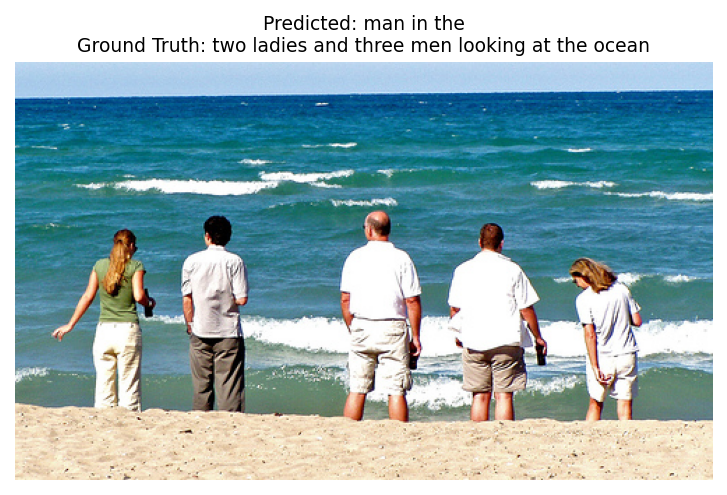
\includegraphics[width=0.7\textwidth]{baseline_example.png}
  \caption{Esempio 1: output rappresentativo della configurazione baseline.}
\end{figure}

\textbf{Interpretazione.} Nella baseline la didascalia risulta generalmente corretta sul piano grammaticale, ma tende a essere più generica e meno discriminativa. Questo comportamento è coerente con l’uso della CNN congelata, che fornisce feature visive robuste ma non ancora adattate in modo ottimale al dominio specifico del dataset. La frase prodotta, quindi, appare plausibile ma più vicina a uno schema descrittivo frequente che a una vera interpretazione fine della scena.

\vspace{0.5em}

\begin{figure}[H]
  \centering
  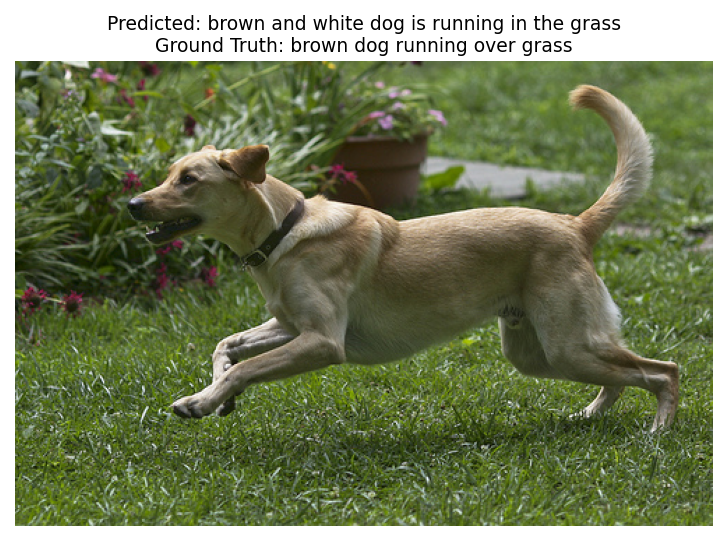
\includegraphics[width=0.7\textwidth]{finetune_example.png}
  \caption{Esempio 2: output qualitativamente riuscito della configurazione con fine-tuning.}
\end{figure}

\textbf{Interpretazione.} Il fine-tuning dell’encoder migliora la specificità della descrizione: il modello coglie meglio il soggetto principale e l’azione dominante, producendo una caption più aderente al contenuto visivo. Questo riscontro qualitativo è pienamente coerente con il miglioramento quantitativo osservato su tutte le metriche BLEU e suggerisce che l’adattamento dell’estrattore visivo produca feature più informative per il decoder linguistico.

\vspace{0.5em}

\begin{figure}[H]
  \centering
  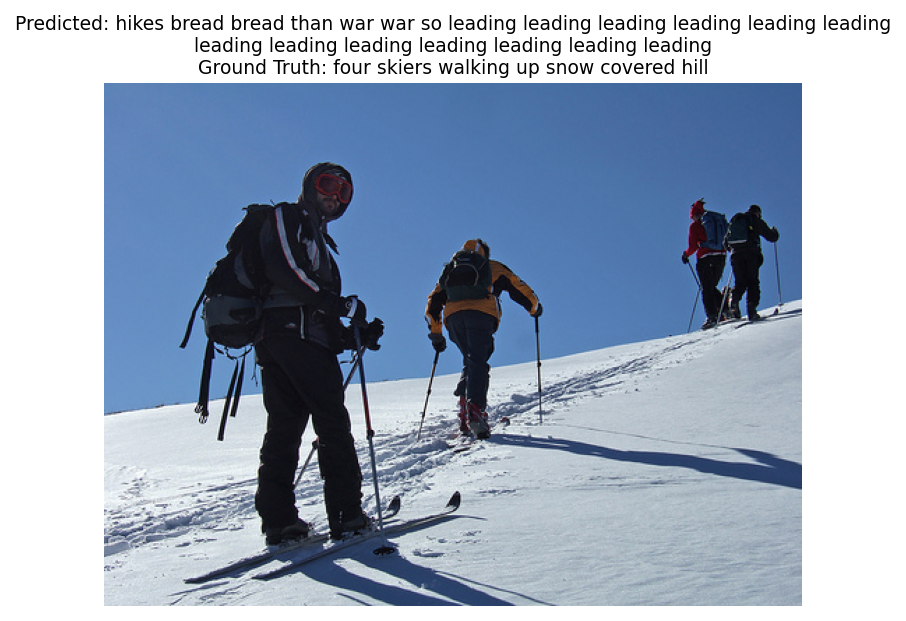
\includegraphics[width=0.7\textwidth]{failure_case.png}
  \caption{Esempio 3: caso di fallimento utile a discutere i limiti del modello.}
\end{figure}

\textbf{Interpretazione.} Nel \emph{failure case} il modello mostra rumore lessicale, ripetizioni o perdita di aderenza semantica. Questo tipo di errore evidenzia un limite tipico delle architetture ricorrenti in compiti di generazione: la tendenza a collassare su sequenze ad alta frequenza o a degradare quando la rappresentazione visiva non fornisce un segnale sufficientemente discriminante. L’inclusione di questo esempio è importante perché evita di costruire una valutazione qualitativa basata esclusivamente sui casi migliori.

\begin{tcolorbox}[title=Osservazione]
L'analisi qualitativa completa quella quantitativa. Il modello è in grado di produrre caption spesso plausibili e sintatticamente corrette, ma la differenza tra baseline e fine-tuning emerge soprattutto nella precisione con cui viene selezionato il contenuto saliente dell’immagine. I casi di fallimento restano fondamentali, perché mostrano che il miglioramento numerico non elimina del tutto fenomeni di genericità, ripetizione o descrizione incompleta.
\end{tcolorbox}

\section{Grafici di training}

Per monitorare l’apprendimento sono stati utilizzati i log di training e validation prodotti dal progetto. Nella versione finale del repository non sono stati conservati grafici esportati completi per tutte le run; di conseguenza, l’analisi seguente si basa sui valori realmente presenti nei log e nei riepiloghi degli esperimenti. Anche in assenza di una visualizzazione uniforme per tutte le configurazioni, i log permettono comunque di ricostruire il comportamento relativo delle diverse strategie di addestramento.

\begin{tcolorbox}[title=Interpretazione dei grafici]
\begin{itemize}
  \item La baseline termina con \texttt{final\_train\_loss = 4.8016} e \texttt{final\_val\_loss = 4.2332}, mentre la migliore validation loss della run è pari a 4.1927.
  \item Le ablation senza scheduled sampling e senza label smoothing mostrano loss di validazione anche migliori della baseline, ma ottengono BLEU inferiori: ciò conferma che la sola loss non è sufficiente a valutare la qualità di un modello generativo.
  \item Il fine-tuning della CNN porta al miglior BLEU-4 dell'intera campagna (\textbf{0.0649}), anche se non coincide con la loss finale più bassa. Questo dato è importante perché mostra una differenza concreta tra ottimizzazione del training e qualità testuale finale.
\end{itemize}
\end{tcolorbox}

\section{Discussione dei limiti}

Nonostante il buon comportamento relativo della configurazione migliore, il modello CNN–LSTM presenta alcuni limiti strutturali che emergono con chiarezza sia dai punteggi quantitativi sia dagli esempi qualitativi:
\begin{itemize}
  \item dipende fortemente dalla qualità delle caption di training;
  \item fatica a descrivere relazioni complesse tra oggetti (es. “il bambino accanto al cane”);
  \item genera frasi talvolta ripetitive o generiche (“a man standing on a street”).
\end{itemize}

Questi limiti non devono essere letti come un fallimento del progetto, ma come conseguenze prevedibili del setting sperimentale adottato. Il dataset è relativamente piccolo, il decoder è ricorrente e la generazione avviene senza tecniche di decoding più ricche come beam search. In questo quadro, la capacità del modello di produrre didascalie plausibili resta significativa, ma non elimina i problemi di specificità lessicale e di rappresentazione delle relazioni più sottili.

\begin{tcolorbox}[title=Cause e possibili soluzioni]
\begin{itemize}
  \item L’uso di un decoder \textbf{Transformer} potrebbe migliorare la modellazione del contesto linguistico.
  \item L’addestramento con una funzione di perdita basata su \textbf{CIDEr} o metodi di \textbf{Reinforcement Learning} permetterebbe di ottimizzare direttamente la qualità linguistica.
  \item L’ampliamento del dataset (es. MSCOCO) favorirebbe una migliore generalizzazione.
\end{itemize}
\end{tcolorbox}

\section{Conclusioni del capitolo}

In sintesi, la valutazione del modello CNN–LSTM mostra che:
\begin{itemize}
  \item il sistema è in grado di generare descrizioni plausibili e coerenti con il contenuto visivo;
  \item scheduled sampling e label smoothing contribuiscono in modo positivo alla generalizzazione del decoder;
  \item il fine-tuning della CNN rappresenta la variante più efficace nel setup sperimentale adottato.
\end{itemize}

Nel complesso, la sezione sperimentale conferma che il progetto non si limita a implementare una pipeline formalmente corretta, ma consente anche di osservare relazioni metodologicamente sensate tra scelte di training e qualità delle didascalie generate. In questo senso, il capitolo di valutazione costituisce uno dei punti più forti dell’elaborato, perché mostra in modo verificabile quali componenti abbiano effettivamente inciso sulle prestazioni finali.

\begin{tcolorbox}[title=Riferimento al codice]
Gli script utilizzati per la valutazione e la generazione delle didascalie sono disponibili nei file:
\begin{itemize}
  \item \texttt{src/eval.py} – calcolo delle metriche BLEU;
  \item \texttt{src/visualize.py} – generazione e salvataggio delle immagini con caption predetta;
  \item \texttt{logs/} e \texttt{results/} – log di training, riepiloghi numerici e predizioni salvate per ciascun esperimento.
\end{itemize}
\end{tcolorbox}

\chapter{Conclusioni e Prospettive Future}

\section{Sintesi del lavoro svolto}

Il progetto ha avuto come obiettivo la realizzazione di un sistema completo di \emph{image captioning} basato su architettura \textbf{CNN--LSTM}, capace di generare descrizioni testuali a partire da immagini e di essere valutato con un protocollo sperimentale esplicito. La pipeline sviluppata comprende la preparazione del dataset, la costruzione del vocabolario, l'implementazione del modello, l'addestramento con diverse configurazioni e l'analisi quantitativa e qualitativa dei risultati.

L’intero percorso ha attraversato tutte le fasi fondamentali di un progetto di deep learning:
\begin{itemize}
  \item analisi del problema e definizione della pipeline \emph{image-to-sequence};
  \item preparazione e pulizia del dataset \dataset{};
  \item estrazione delle feature visive tramite CNN pre-addestrata (InceptionV3);
  \item modellazione linguistica mediante LSTM e embedding trainabili;
  \item addestramento supervisionato con teacher forcing, scheduled sampling e label smoothing;
  \item valutazione quantitativa e qualitativa dei risultati ottenuti.
\end{itemize}

\begin{tcolorbox}[title=Risultato principale]
La migliore configurazione sperimentale del progetto è risultata quella con fine-tuning della CNN, che ha raggiunto un punteggio \textbf{BLEU-4 pari a 0.0649}. Pur rimanendo lontano dalle prestazioni dei modelli più avanzati della letteratura, questo risultato conferma la coerenza della pipeline implementata e mostra un miglioramento netto rispetto alla baseline e alle ablation prive di scheduled sampling o label smoothing.
\end{tcolorbox}

\section{Contributi e aspetti innovativi}

Tra gli aspetti qualificanti di questo lavoro si evidenziano:
\begin{itemize}
  \item l’implementazione modulare in PyTorch, con codice leggibile e ampiamente commentato;
  \item l’uso di tecniche di stabilizzazione come gradient clipping e label smoothing;
  \item l’applicazione di \textbf{scheduled sampling} per migliorare la robustezza del decoder LSTM;
  \item l’utilizzo di 5 caption per immagine nella valutazione BLEU, rendendo la metrica più affidabile;
  \item la visualizzazione interattiva dei risultati tramite interfaccia Streamlit.
\end{itemize}

Nel complesso, questi elementi rendono il progetto riproducibile, facilmente ispezionabile e adatto a successive estensioni sperimentali. Il contributo più concreto non è tanto l'adozione di una singola tecnica, quanto la costruzione di una pipeline coerente in cui ciascuna scelta può essere verificata e discussa alla luce dei risultati ottenuti.

\section{Limiti riscontrati}

I risultati ottenuti mostrano anche con chiarezza alcuni limiti strutturali del modello CNN--LSTM adottato:
\begin{itemize}
  \item la difficoltà nel catturare relazioni complesse tra oggetti e azioni;
  \item la tendenza a produrre frasi grammaticalmente corrette ma poco varie;
  \item la dipendenza da dataset relativamente piccoli come Flickr8k;
  \item la mancanza di attenzione visiva (il modello non “guarda” regioni specifiche dell’immagine).
\end{itemize}

\begin{tcolorbox}[title=Analisi critica]
Questi limiti derivano in gran parte dalla natura sequenziale del decoder LSTM, dall'assenza di un meccanismo di attenzione visiva esplicito e dalla dimensione ridotta del dataset. In un contesto di progetto, tali vincoli non invalidano il lavoro svolto, ma definiscono con precisione l'ambito entro cui i risultati devono essere interpretati.
\end{tcolorbox}

\section{Prospettive future}

Le estensioni più naturali del progetto riguardano sia l'architettura sia la strategia di valutazione:
\begin{itemize}
  \item sostituzione del decoder LSTM con un \textbf{Transformer decoder}, in grado di gestire contesti più lunghi e paralleli;
  \item introduzione di un \textbf{meccanismo di attenzione visiva} per localizzare oggetti rilevanti nell’immagine;
  \item addestramento con metodi di \textbf{Reinforcement Learning} per ottimizzare metriche linguistiche (CIDEr, SPICE);
  \item espansione a dataset più ampi e complessi (MSCOCO, Flickr30k);
  \item sviluppo di un sistema multimodale in tempo reale integrabile in applicazioni di accessibilità visiva.
\end{itemize}

\begin{tcolorbox}[title=Confronto concettuale con modelli più recenti]
L'architettura CNN--LSTM impiegata in questo progetto rappresenta una soluzione classica, oggi meno competitiva rispetto agli approcci basati su attenzione e Transformer, ma ancora estremamente utile per studiare in modo trasparente il legame tra rappresentazione visiva, modellazione sequenziale e qualità delle caption generate. In questo senso, il modello adottato costituisce una base metodologica solida da cui partire per confronti futuri con architetture più recenti.
\end{tcolorbox}

\section{Conclusione generale}

Nel complesso, il lavoro svolto documenta un percorso completo di progettazione, sviluppo e valutazione di un sistema di \emph{image captioning}. Il valore del progetto non risiede soltanto nell'implementazione dell'architettura CNN--LSTM, ma soprattutto nella possibilità di osservare in modo verificabile come diverse scelte di training influenzino la qualità finale delle descrizioni generate. Da questo punto di vista, la campagna sperimentale ha fornito un risultato chiaro: scheduled sampling, label smoothing e fine-tuning dell'encoder non sono dettagli marginali, ma componenti che incidono concretamente sul comportamento del modello.

\begin{tcolorbox}[title=Considerazione finale]
Il progetto fornisce una base affidabile per ulteriori sviluppi nel captioning multimodale. Pur collocandosi entro un setting sperimentale contenuto, esso mostra come una pipeline ben costruita, correttamente documentata e supportata da risultati reali possa costituire un elaborato solido e tecnicamente difendibile.
\end{tcolorbox}

\chapter{Analisi dei file e delle funzioni implementate}

In questa sezione viene fornita una descrizione dettagliata delle componenti software sviluppate per il progetto di \emph{Image Captioning} basato su architettura CNN--LSTM.  
L'obiettivo è illustrare in modo chiaro le funzioni principali di ciascun file, spiegandone il ruolo, la logica interna e le interazioni con le altre parti del sistema.  
Tutti i file sono scritti in linguaggio Python e utilizzano il framework PyTorch per la modellazione neurale.

\section{File \texttt{vocab\_builder.py}}

Questo modulo si occupa della costruzione del vocabolario testuale a partire dalle caption del dataset.  
Le funzioni principali sono:

\begin{itemize}
  \item \textbf{clean\_caption(caption)} – Pulisce una singola caption rendendola uniforme: converte il testo in minuscolo, rimuove punteggiatura, numeri e parole isolate, restituendo una stringa pulita pronta per la tokenizzazione.
  \item \textbf{build\_vocabulary(captions, min\_freq)} – Crea un dizionario di parole (vocabolo–indice) contando la frequenza di ogni termine. Solo le parole che appaiono almeno \texttt{min\_freq} volte vengono incluse per ridurre la dimensione del vocabolario.
  \item \textbf{save\_vocabulary(vocab, path)} – Salva il vocabolario in formato JSON per essere caricato successivamente durante il training.
  \item \textbf{load\_vocabulary(path)} – Carica un vocabolario salvato in precedenza da file.
\end{itemize}

Questo file è il primo passo del processo, poiché produce il dizionario token–indice necessario per convertire le caption testuali in sequenze numeriche gestibili dalla rete LSTM.

\section{File \texttt{dataset.py}}

Definisce la classe \texttt{FlickrDataset}, che eredita da \texttt{torch.utils.data.Dataset} e gestisce l'associazione tra immagini e caption.  
Le funzioni principali sono:

\begin{itemize}
  \item \textbf{\_\_init\_\_} – Inizializza il dataset, caricando le informazioni da un file CSV contenente i nomi delle immagini e le caption. Riceve anche il dizionario del vocabolario e le trasformazioni da applicare alle immagini.
  \item \textbf{\_\_getitem\_\_(index)} – Restituisce una coppia immagine–caption alla posizione specificata. L’immagine viene caricata e trasformata (resize, normalizzazione), mentre la caption viene convertita in una sequenza di indici, con l’aggiunta dei token speciali \bos{} e \eos{}.
  \item \textbf{\_\_len\_\_} – Restituisce la lunghezza del dataset, utile per il DataLoader PyTorch.
\end{itemize}

Questo modulo è il ponte tra i dati grezzi e la rete neurale, preparando batch coerenti di immagini e testo per il training.

\section{File \texttt{model.py}}

Contiene la definizione dell'architettura neurale CNN–LSTM e rappresenta il cuore del progetto.  
Le funzioni principali sono:

\begin{itemize}
  \item \textbf{EncoderCNN} – Classe che utilizza una CNN pre-addestrata (InceptionV3 o ResNet50) per estrarre feature visive dall’immagine. Rimuove gli strati di classificazione finali e aggiunge una proiezione lineare per ridurre la dimensionalità delle feature.
  \item \textbf{DecoderLSTM} – Classe che definisce la rete ricorrente (LSTM) e un layer fully connected che mappa lo stato nascosto sull’intero vocabolario, producendo una distribuzione di probabilità sulle parole successive.
  \item \textbf{forward(image, caption)} – Descrive il passaggio in avanti: le feature estratte dalla CNN vengono fornite alla LSTM, che genera la sequenza testuale passo per passo.
  \item \textbf{sample(features)} – Metodo usato in fase di test per generare una caption, parola dopo parola, partendo solo dalle feature visive.
\end{itemize}

\section{File \texttt{train.py}}

Implementa la logica di addestramento del modello e la gestione delle epoche.  
Le funzioni principali includono:

\begin{itemize}
  \item \textbf{train\_one\_epoch(model, dataloader, optimizer, criterion)} – Esegue un’epoca di addestramento: calcola la perdita, effettua il backpropagation e aggiorna i pesi.
  \item \textbf{evaluate(model, val\_loader)} – Valuta il modello sul set di validazione, restituendo la perdita media e (facoltativamente) la metrica BLEU.
  \item \textbf{save\_checkpoint(state, path)} – Salva lo stato corrente del modello (pesi, epoca, ottimizzatore).
  \item \textbf{train()} – Funzione principale che gestisce il ciclo di addestramento completo, l’aggiornamento del learning rate, il salvataggio dei migliori pesi e l’applicazione dello \emph{scheduled sampling}.
\end{itemize}

\section{File \texttt{eval.py}}

Questo script esegue la valutazione del modello addestrato e genera caption per le immagini di test.  
Le funzioni chiave sono:

\begin{itemize}
  \item \textbf{generate\_caption(model, image)} – Utilizza il metodo \texttt{sample()} del decoder per produrre una frase descrittiva a partire da un’immagine.
  \item \textbf{compute\_bleu(references, predictions)} – Calcola la metrica BLEU confrontando le caption predette con quelle reali, utilizzando tutte le 5 descrizioni disponibili per ogni immagine.
  \item \textbf{evaluate\_model(model, test\_loader)} – Esegue la valutazione completa sull’intero dataset di test, restituendo il punteggio BLEU complessivo e salvando i risultati.
\end{itemize}

\section{File \texttt{visualize.py}}

Si occupa di mostrare esempi qualitativi di caption generate.  
Carica un sottoinsieme di immagini, genera le rispettive descrizioni e le salva in un’unica figura comparativa (immagine + caption reale + caption predetta).  
Include inoltre una funzione per creare overlay grafici direttamente sull’immagine.

\section{File \texttt{ui\_streamlit.py}}

Contiene una semplice interfaccia utente sviluppata con Streamlit, che consente di caricare un’immagine e ottenere in tempo reale la didascalia generata dal modello.  
Le funzioni principali sono:

\begin{itemize}
  \item \textbf{load\_model(weights\_path)} – Carica i pesi del modello addestrato.
  \item \textbf{predict\_caption(image)} – Esegue la generazione della didascalia a partire da un’immagine fornita dall’utente.
  \item \textbf{main()} – Crea l’interfaccia grafica, gestendo il caricamento delle immagini e la visualizzazione dei risultati.
\end{itemize}

\section{File \texttt{utils.py}}

Contiene funzioni di supporto comuni a più moduli:
\begin{itemize}
  \item \textbf{set\_seed(seed)} – Imposta un seme casuale per rendere gli esperimenti riproducibili.
  \item \textbf{save\_config(config)} – Salva le configurazioni di training in un file YAML.
  \item \textbf{count\_parameters(model)} – Restituisce il numero totale di parametri addestrabili del modello.
  \item \textbf{decode\_tokens(tokens, vocab)} – Converte una sequenza di indici numerici nella corrispondente sequenza di parole.
\end{itemize}

---

Insieme, questi moduli costituiscono un sistema completo e modulare per l’addestramento, la valutazione e l’utilizzo di un modello di \emph{image captioning} basato su CNN–LSTM.  
Ogni file ha un ruolo specifico e interagisce con gli altri tramite interfacce chiare e ben definite, in modo da garantire manutenibilità e riutilizzabilità del codice.






\appendix
\chapter{Struttura del Repository e Istruzioni d'Uso}

\section{Repository GitHub del progetto}

Il codice sorgente completo, i file di configurazione e gli artefatti di addestramento sono disponibili nel repository ufficiale del progetto:

\begin{tcolorbox}[colback=gray!5!white, colframe=gray!70!black, title=Repository ufficiale]
\url{https://github.com/giuseppedimonte/image-captioning-cnn-lstm}
\end{tcolorbox}

Il repository è pubblico e contiene tutto il materiale necessario per eseguire, testare e valutare il modello.  
È strutturato in modo modulare per facilitare la comprensione, la riproducibilità e l'estensione del lavoro.

\section{Struttura delle cartelle}

\begin{verbatim}
image-captioning-cnn-lstm/
|
|-- src/                     # Codice sorgente principale
|   |-- dataset.py           # Gestione del dataset e preprocessing
|   |-- model.py             # Definizione del modello CNN-LSTM
|   |-- train.py             # Script di addestramento
|   |-- eval.py              # Script di valutazione (BLEU)
|   |-- visualize.py         # Generazione e visualizzazione caption
|   |-- vocab_builder.py     # Creazione del dizionario token-indice
|   \-- utils.py             # Funzioni di supporto
|
|-- configs/                 # File di configurazione
|   |-- config.yml           # Configurazione generale del progetto
|   |-- baseline_cpu.yml
|   |-- ablation_no_scheduled_sampling_cpu.yml
|   |-- ablation_no_label_smoothing_cpu.yml
|   \-- ablation_finetune_cpu.yml
|
|-- checkpoints/             # Pesi salvati dei modelli
|   |-- baseline_cpu/
|   |-- ablation_no_ss_cpu/
|   |-- ablation_no_ls_cpu/
|   \-- ablation_finetune_cpu/
|
|-- logs/                    # Log testuali di training ed evaluation
|-- results/                 # Predizioni e riepiloghi metrici
|
|-- figures/                 # Immagini e grafici per il report
|
|-- requirements.txt         # Dipendenze Python
|-- README.md                # Documentazione del progetto
\-- LICENSE                  # Licenza open-source (MIT)
\end{verbatim}

\begin{tcolorbox}[title=Nota]
La struttura è progettata per rispettare le buone pratiche di sviluppo in PyTorch e per garantire la riproducibilità dei risultati.
\end{tcolorbox}

\section{Installazione e requisiti}

\subsection{Requisiti di sistema}
\begin{itemize}
  \item Python 3.10 o superiore
  \item PyTorch $\geq$ 2.0 con supporto CUDA (GPU opzionale ma consigliata)
  \item NLTK, NumPy, Pillow, Matplotlib, PyYAML
\end{itemize}

\subsection{Installazione passo per passo}

\begin{verbatim}
# Clonare il repository
git clone https://github.com/giuseppedimonte/image-captioning-cnn-lstm.git
cd image-captioning-cnn-lstm

# Creare un ambiente virtuale
python -m venv venv
source venv/bin/activate   # (Linux/Mac)
venv\Scripts\activate      # (Windows)

# Installare le dipendenze
pip install -r requirements.txt
\end{verbatim}

\begin{tcolorbox}[title=Suggerimento]
Per eseguire l'addestramento su GPU è consigliato verificare la corretta installazione di \texttt{torch.cuda.is\_available()}.
\end{tcolorbox}

\section{Esecuzione del training}

L’addestramento del modello può essere lanciato direttamente tramite terminale. Nel protocollo sperimentale finale, la configurazione di riferimento utilizzata è stata la baseline CPU:

\begin{verbatim}
python src/train.py --config configs/baseline_cpu.yml
\end{verbatim}

Durante l’addestramento, verranno generati:
\begin{itemize}
  \item log testuali in \texttt{logs/};
  \item checkpoint nelle sottocartelle di \texttt{checkpoints/};
  \item predizioni e riepiloghi metrici in \texttt{results/}.
\end{itemize}

\begin{tcolorbox}[title=Esempio di configurazione YAML]
\begin{verbatim}
train:
  batch_size: 16
  epochs: 5
  learning_rate: 0.0005
  teacher_forcing_start: 0.7
  teacher_forcing_end: 0.3
  label_smoothing: 0.1
model:
  embed_dim: 256
  hidden_dim: 512
  dropout: 0.3
\end{verbatim}
\end{tcolorbox}

\section{Valutazione e generazione caption}

Per valutare il modello addestrato e generare nuove caption:

\begin{verbatim}
python src/eval.py --images_dir data/Flickr8k_Dataset \
  --captions_json data/Flickr8k_text/test_captions.json \
  --vocab_path data/vocab.json \
  --weights checkpoints/baseline_cpu/model_best.pt
\end{verbatim}

Le didascalie prodotte verranno salvate in formato JSON o CSV e potranno essere visualizzate con:
\begin{verbatim}
python src/visualize.py --weights checkpoints/baseline_cpu/model_best.pt \
  --vocab_path data/vocab.json \
  --images_dir data/Flickr8k_Dataset \
  --captions_json data/Flickr8k_text/test_captions.json \
  --output_dir figures/baseline_cpu
\end{verbatim}

\section{Esecuzione dell’interfaccia Streamlit}

L’interfaccia utente, sviluppata con Streamlit, permette di caricare un’immagine e visualizzare la caption generata in tempo reale:

\begin{verbatim}
streamlit run src/ui_streamlit.py
\end{verbatim}

\begin{tcolorbox}[title=Esempio d’uso]
Caricare un file immagine dal browser, attendere l’elaborazione e visualizzare la didascalia proposta dal modello.  
L’interfaccia permette di verificare in tempo reale il comportamento del modello su nuove immagini, costituendo un supporto qualitativo utile accanto alla valutazione quantitativa.
\end{tcolorbox}

\section{Riproducibilità dei risultati}

Per garantire risultati ripetibili:
\begin{itemize}
  \item impostare il seme casuale globale (\texttt{torch.manual\_seed(42)});
  \item salvare il file di configurazione utilizzato;
  \item annotare il numero di epoche, la GPU usata e la versione di PyTorch.
\end{itemize}

\begin{tcolorbox}[title=Buone pratiche finali]
Il repository è organizzato secondo principi di riproducibilità e tracciabilità.  
Tutti i risultati principali (punteggi BLEU, immagini qualitative, log di training ed evaluation, predizioni JSON) sono documentati e archiviati per verifica.
\end{tcolorbox}


\chapter*{Appendice B – Glossario dei Termini Tecnici}
\addcontentsline{toc}{chapter}{Appendice B – Glossario dei Termini Tecnici}

\section*{Introduzione}

Questa appendice raccoglie e spiega in modo sintetico ma preciso i principali concetti e termini tecnici utilizzati nel progetto.  
Il glossario ha lo scopo di fornire una visione chiara e unificata delle componenti che concorrono al funzionamento del sistema di \emph{image captioning} basato su CNN–LSTM.

\bigskip

\begin{description}

  \item[\textbf{Addestramento (Training)}]  
  Processo mediante il quale una rete neurale apprende dai dati, ottimizzando i propri parametri interni (pesi e bias) per ridurre l’errore tra le predizioni e i valori attesi.

  \item[\textbf{Batch}]  
  Insieme di campioni elaborati contemporaneamente durante un passo dell’addestramento.  
  L’uso dei batch migliora la stabilità e l’efficienza computazionale del training.

  \item[\textbf{BLEU (Bilingual Evaluation Understudy)}]  
  Metrica di valutazione per la generazione di testo.  
  Misura la sovrapposizione di sequenze di parole (\emph{n-grammi}) tra la frase generata e quelle di riferimento, penalizzando caption troppo corte.

  \item[\textbf{CNN (Convolutional Neural Network)}]  
  Architettura neurale specializzata nell’elaborazione di immagini.  
  Utilizza operazioni di convoluzione per rilevare pattern locali come bordi, texture e forme.

  \item[\textbf{Caption}]  
  Descrizione testuale che sintetizza il contenuto di un’immagine.  
  Nel contesto del progetto, è la sequenza di parole generata dal modello a partire da un input visivo.

  \item[\textbf{Dataset}]  
  Insieme di dati (immagini e descrizioni) utilizzato per addestrare e valutare il modello.  
  In questo progetto viene impiegato il dataset \dataset{}, che contiene 8.000 immagini e 5 descrizioni per ciascuna.

  \item[\textbf{Embedding}]  
  Rappresentazione vettoriale densa di parole o immagini.  
  Nel caso del linguaggio naturale, ogni parola è associata a un vettore numerico che cattura relazioni semantiche e sintattiche.

  \item[\textbf{Epoca (Epoch)}]  
  Un’epoca corrisponde a un passaggio completo del modello su tutto il dataset di addestramento.  
  L’apprendimento avviene gradualmente su più epoche, fino a convergere.

  \item[\textbf{Feature (Caratteristica)}]  
  Informazione numerica estratta da un’immagine (es. presenza di forme, colori, texture).  
  Le feature sono la base su cui la LSTM genera le descrizioni.

  \item[\textbf{Fine-tuning}]  
  Tecnica che consiste nell’adattare un modello pre-addestrato (ad esempio una CNN) a un nuovo compito, modificando solo gli ultimi strati.  
  Permette di ridurre i tempi di addestramento e migliorare le prestazioni su dataset piccoli.

  \item[\textbf{Gradient Clipping}]  
  Tecnica di stabilizzazione che limita l’ampiezza dei gradienti durante la retropropagazione.  
  Serve a evitare che valori troppo grandi causino instabilità numerica o blocchi nel training.

  \item[\textbf{Hidden State (Stato Nascosto)}]  
  Rappresentazione interna mantenuta dalla LSTM a ogni passo temporale.  
  Contiene informazioni sul contesto linguistico accumulato fino a quel punto della sequenza.

  \item[\textbf{LSTM (Long Short-Term Memory)}]  
  Variante delle reti ricorrenti (RNN) capace di modellare dipendenze a lungo termine grazie all’uso di tre porte: input, forget e output.  
  È il cuore della generazione di testo nel modello proposto.

  \item[\textbf{Loss Function (Funzione di Perdita)}]  
  Misura la differenza tra l’output del modello e il valore corretto.  
  Nel progetto è utilizzata la \emph{Cross Entropy Loss}, comune nei problemi di classificazione.

  \item[\textbf{Overfitting}]  
  Fenomeno per cui un modello impara eccessivamente i dati di training, perdendo capacità di generalizzazione.  
  Si controlla con tecniche come dropout, early stopping e data augmentation.

  \item[\textbf{Scheduled Sampling}]  
  Strategia che riduce progressivamente il \emph{teacher forcing}, abituando il modello a usare le proprie predizioni durante l’addestramento.  
  Migliora la robustezza e la naturalezza delle frasi generate.

  \item[\textbf{Teacher Forcing}]  
  Tecnica in cui, durante il training, la parola corretta (ground truth) viene fornita come input successivo alla LSTM, invece della parola predetta.  
  Accelerando l’apprendimento ma riducendo la robustezza al test.

  \item[\textbf{Token}]  
  Unità linguistica elementare (parola o simbolo) in cui viene scomposto un testo.  
  I token vengono numericamente codificati tramite un dizionario (\emph{vocab}).

  \item[\textbf{Transfer Learning}]  
  Metodo che sfrutta le conoscenze di un modello pre-addestrato su un grande dataset per un nuovo compito.  
  In questo progetto, la CNN (InceptionV3) è stata usata come estrattore di feature pre-addestrato su ImageNet.

  \item[\textbf{Transformer}]  
  Architettura neurale basata su meccanismi di attenzione, oggi dominante nel campo dell’IA multimodale.  
  È considerata l’evoluzione naturale delle RNN e LSTM, capace di elaborare sequenze in parallelo.

\end{description}

\bigskip
\noindent
\textit{Questo glossario intende offrire una visione d’insieme chiara e rigorosa dei concetti fondamentali trattati nel progetto, fungendo da supporto alla comprensione dei capitoli tecnici.}


\chapter*{Appendice C – Timeline del Progetto e Riproducibilità degli Esperimenti}
\addcontentsline{toc}{chapter}{Appendice C – Timeline del Progetto e Riproducibilità degli Esperimenti}

\section*{Introduzione}

Questa appendice documenta il percorso di sviluppo del progetto, illustrando le principali fasi, le attività svolte in ciascun momento e le procedure adottate per garantire la riproducibilità completa degli esperimenti.

\section{Timeline del progetto}

La seguente tabella riassume le tappe fondamentali del progetto, dalla fase iniziale di analisi alla presentazione finale.

\begin{table}[H]
\centering
\begin{tabular}{@{}llp{8cm}@{}}
\toprule
\textbf{Fase} & \textbf{Descrizione} & \textbf{Attività principali} \\ \midrule
Analisi iniziale & Comprensione del problema & Studio del dataset Flickr8k, revisione della letteratura sui modelli CNN–LSTM, definizione degli obiettivi del progetto. \\
Progettazione & Definizione dell'architettura & Pianificazione della pipeline image-to-sequence, scelta dei parametri principali e struttura del repository. \\
Implementazione & Sviluppo del codice & Creazione del dataloader, preprocessing del testo, costruzione del vocabolario e definizione del modello CNN–LSTM in PyTorch. \\
Addestramento & Ottimizzazione dei parametri & Esecuzione degli esperimenti, tuning degli iperparametri, monitoraggio della perdita e salvataggio dei checkpoint. \\
Valutazione & Analisi delle prestazioni & Calcolo delle metriche BLEU, analisi qualitativa delle caption e confronto tra diverse configurazioni. \\
Visualizzazione & Presentazione dei risultati & Creazione di grafici, immagini esemplificative e sviluppo dell’interfaccia Streamlit per la generazione in tempo reale. \\
Documentazione finale & Sintesi e revisione & Stesura del report accademico, commento del codice e preparazione della discussione orale. \\ \bottomrule
\end{tabular}
\caption{Fasi principali del progetto e relative attività.}
\end{table}

\section{Controllo di versione e tracciabilità}

Per garantire trasparenza e riproducibilità, il codice è stato gestito tramite \textbf{Git} e pubblicato su GitHub con commit regolari.  
Ogni commit corrisponde a una modifica coerente (nuova funzionalità, correzione, esperimento o aggiornamento documentale) ed è accompagnato da un messaggio standardizzato:

\begin{verbatim}
feat: add scheduled sampling in training loop
fix: correct BLEU score computation in eval.py
docs: update README with installation instructions
\end{verbatim}

Inoltre, ogni esperimento è stato eseguito utilizzando un file di configurazione YAML dedicato, contenente tutti i parametri di training (learning rate, batch size, numero di epoche, dropout, ecc.), archiviato nella directory \texttt{configs/}.

\section{Riproducibilità degli esperimenti}

Per replicare gli esperimenti descritti nel documento:

\begin{enumerate}
  \item Clonare il repository del progetto.
  \item Installare le dipendenze elencate in \texttt{requirements.txt}.
  \item Scaricare e posizionare il dataset Flickr8k nella cartella \texttt{data/}.
  \item Avviare l’addestramento con:
  \begin{verbatim}
  python src/train.py --config configs/baseline_cpu.yml
  \end{verbatim}
  \item Valutare il modello addestrato:
  \begin{verbatim}
  python src/eval.py --images_dir data/Flickr8k_Dataset --captions_json data/Flickr8k_text/test_captions.json --vocab_path data/vocab.json --weights checkpoints/baseline_cpu/model_best.pt
  \end{verbatim}
  \item Visualizzare le caption generate:
  \begin{verbatim}
  python src/visualize.py --weights checkpoints/baseline_cpu/model_best.pt --vocab_path data/vocab.json --images_dir data/Flickr8k_Dataset --captions_json data/Flickr8k_text/test_captions.json --output_dir figures/baseline_cpu
  \end{verbatim}
\end{enumerate}

\section{Suggerimenti pratici per la replica}

\begin{itemize}
  \item Utilizzare un ambiente virtuale o \texttt{conda} per evitare conflitti di versione.
  \item Impostare un seme casuale fisso per garantire la comparabilità dei risultati.
  \item Salvare log testuali e riepiloghi metrici per ogni esperimento.
  \item Eseguire test con diversi learning rate (es. 0.001, 0.0005, 0.0001) e documentare le differenze di prestazione.
  \item Mantenere una cartella separata per ciascun esperimento (\texttt{exp1}, \texttt{exp2}, ecc.) con i relativi file di configurazione e pesi.
\end{itemize}

\section{Conclusione}

Il processo di sviluppo e validazione del modello è stato pianificato e tracciato con attenzione, in modo da garantire che ogni risultato riportato sia verificabile e riproducibile.  
Questa appendice fornisce le informazioni necessarie per replicare integralmente gli esperimenti e proseguire con ulteriori miglioramenti o confronti futuri.


\end{document}
